\chapter{Graph analysis}
% todo citare documentazione di neo4j
\section{Prescription coupling}
An excessive usage of antibiotics causes death of microorganisms in the human body which provide to maintaining immune cells and killing certain oral infections\cite{bacteria}.

To equilibrate the intestinal flora, lactic ferments are often taken together with antibiotics, so that new ``good'' bacteria can restore the probiotic action.

If this hypothesis is correct, the dataset will show antibiotic prescriptions paired with other drugs, on the same date --- or it will highlight potential linkings between infections and other pathologies receiving a specific prescription.

\section{Graph databases}
Graph databases are data management systems allowing persistent representation of entity and relationship in a graph structure, implementing the Property Graph Model efficiently down to the storage level. % todo citare le slide di maurino

A graph $G\: =\: <E, V>$ is an abstract data type showing connections (edges $E$) between pairs of vertices ($V$). Nodes identify entities and their properties, while relationships are joining attributes between tables with eventual additional characteristics. 

Queries allow to match pattern of nodes and relationships in a graph, providing ACID transaction compliance without specifying details on how to implement operations. Graph-crossing and related algorithms are highly efficient.

\section{Goals}
Goals of analytics through graphs is completion of antibiotic patterns changes and patient journey, providing a different point of view on those two important aspects altogether.

This part of the research aims to focus on:
\begin{itemize}
	\item Co-prescriptions, understanding whether specified couples of drugs are often prescribed together;
	\item Clustering, to identify similar kinds of patients according to their prescription history;
	\item Centrality measures of nodes, to highlight particularly important entities in the graph.
\end{itemize}

\section{Practical approach}

\subsection{Relational database structure}
The available data comprehends patients, general practitioners, and their prescriptions in the time span from 2000 to 2018. Summarising the amount of records for each entity:
\begin{itemize}
	\item 888 219 patients;
	\item 2 486 doctors;
	\item 118 716 403 prescriptions;
	\item 33 523 drugs.
\end{itemize}

Due to the amount and veracity of data, identifying a subset of records is useful to have detailed and targeted results, removing dispersive information and leaving a restricted pool of prescriptions, setting acceptability conditions. 

Since analytics are aimed to identify antibiotic prescription patterns, similarly to previous work a new dataset has been extracted, imposing the following constraints:
\begin{enumerate}
	\item AIC corresponding to an antibiotic;
	\item Prescription date between 2008-01-01 and 2017-12-31;
	\item Active general practitioners;
	\item Patients with usable information about sex, date of birth and location.
\end{enumerate}

This leads to obtaining a new relationship, composed by:
\begin{itemize}
	\item 670 634 patients;
	\item 1 377 doctors;
	\item 8 386 057 prescriptions;
	\item 2 802 antibiotics.
\end{itemize}

To allow analytics on patient journey and co-prescriptions, it is necessary to access all the prescriptions assigned to all patients belonging in the subset. A major extraction is performed from the main table, comprehending:
\begin{enumerate}
	\item Identifier of patients who received at least one other antibiotic prescription;
	\item Prescription date between 2008-01-01 and 2017-12-31.
\end{enumerate}

This reduces the number of other prescriptions, adding drugs not belonging to the antibiotic class. Duplicates, mistakes and empty fields are removed. The final composition of data is:

\begin{itemize}
	\item 670 634 patients;
	\item 1 377 doctors;
	\item 8 328 272 prescriptions of antibiotics;
	\item 2 465 antibiotics;
	\item 7 587 009 other prescriptions;
	\item 21 248 other medicines.
\end{itemize}

% todo grafici

\subsection{Migration of the database and graph modelling}
The database has to be structured following the SQL to Cypher practices and guidelines, assigning nodes and relationships in an appropriate way considering the existing dataset and the related goals.

After having a final version of the data to import, the entity-relationship model translates with the following nodes and attributes:
\begin{itemize}
	\item Patient;
	\begin{itemize}
		\item ID, birthdate, sex;
	\end{itemize}
	\item Doctor;
	\begin{itemize}
		\item ID; % luogo?
	\end{itemize}
	\item Antibiotic;
	\begin{itemize}
		\item AIC code, ATC code, active principle;
	\end{itemize}
	\item Medicine (anything not Antibiotic);
	\begin{itemize}
		\item AIC code, ATC code, active principle;
	\end{itemize}
	\item Prescription;
	\begin{itemize}
		\item patient, doctor, date, drug;
	\end{itemize}
	\item OtherPrescription (not Antibiotic Prescription);
	\begin{itemize}
		\item patient, doctor, date, drug.
	\end{itemize}
\end{itemize}

All nodes are imported, and main indexes are created for optimisation of queries speed. Relationships are then created according to IDs and AIC codes:
\begin{itemize}
	\item Prescription $-$ TO $\rightarrow$ Patient;
	\item Prescription $-$ FROM $\rightarrow$ Doctor;
	\item OtherPrescription $-$ OF $\rightarrow$ Antibiotic;
	\item OtherPrescription $-$ TO $\rightarrow$ Patient;
	\item OtherPrescription $-$ FROM $\rightarrow$ Doctor;
	\item OtherPrescription $-$ OF $\rightarrow$ Medicine.
\end{itemize}

After migrating all elements of the graph database, additional features of Patient representing age is added. Since age changes within years, and the considered timespan is 2008-2017, 10 node properties are created for each patient (age2008, age2009, \dots). %todo

\section{Visualisation and analytics}
\subsection{Sample graph}
A sample graph is obtained using the \texttt{apoc} functions.

\begin{figure}[h]
	\centering
	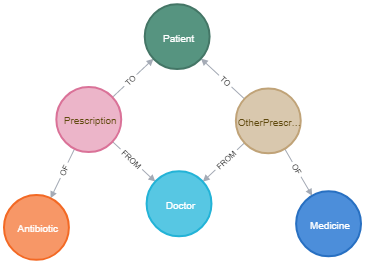
\includegraphics[scale=0.5]{./images/sample-graph.png}
\end{figure}


\subsection{Examples}
An example of graph subset can be obtained extracting one of the individuals with the most antibiotic prescriptions (the 10th in descending order), a male patient born in 1943, and his associated drugs and doctors.

The graph displays:
\begin{enumerate}
	\item 1 patient, the green node in the middle;
	\item 360 antibiotic prescriptions, the pink nodes;
	\item 524 other prescriptions, the brown nodes;
	\item 4 doctors, the light blue nodes;
	\item 25 antibiotics, the orange nodes;
	\item 59 other medicines, the blue nodes. 
\end{enumerate}

\begin{figure}[h]
	\centering
	\includegraphics[scale=0.14]{./images/1-patient-graph.png}
\end{figure}

Having a view focussed on prescriptions, the same procedure is applied extracting the 500th antibiotic in descending order according to number of prescriptions, corresponding to Locabiotal spray bottle 15 ml (50 mg / 5 ml).

The graph displays:
\begin{enumerate}
	\item 1 antibiotic, the orange node in the middle;
	\item 896 antibiotic prescriptions, the pink nodes;
	\item 107 doctors, the light blue nodes;
	\item 817 patients, the green nodes.
\end{enumerate}

\begin{figure}[h]
	\centering
	\includegraphics[scale=0.11]{./images/1-antibiotic-graph.png}
\end{figure}

Those two examples allow to have a general idea of how nodes interact with each other, grouping in clusters. 

\subsection{Graph statistics}
A first set of global and local statistics are used to get the first insight on the graph and its components.

\begin{center}
	\begin{tabular}{c|c}
		Number of nodes & 16 611 005 \\
		\hline
		Number of relationships & 47 745 841 \\
		\hline
		Average prescriptions per doctor & 11 557,93 \\
		\hline
		Standard deviation & 15 457,6 \\
		\hline
		Maximum per doctor & 96 841 \\
		\hline
		Minimum per doctor & 1 \\
		\hline
		Average prescriptions per patient & 23,73 \\
		\hline
		Standard deviation & 40,46 \\
		\hline
		Maximum per patient & 1 567 \\
		\hline
		Minimum per patient & 1
	\end{tabular}
\end{center}

\subsection{Projecting a co-prescription graph}
Since the restriction on generic prescriptions involves having the same date and patient of another antibiotic prescription, couples are analysed adding a relationship between Antibiotic and Medicines in the main graph.

After counting the number of repetitions for each couple Antibiotic-Medicine, the first 100 most popular ones are used to couple nodes, with the amount as property of the relationship PRESCRIBED\_WITH.

Visualising the newly created relationships, two connected components are highlighted (orange antibiotics, blue other medicines).

\begin{figure}[h]
	\centering
	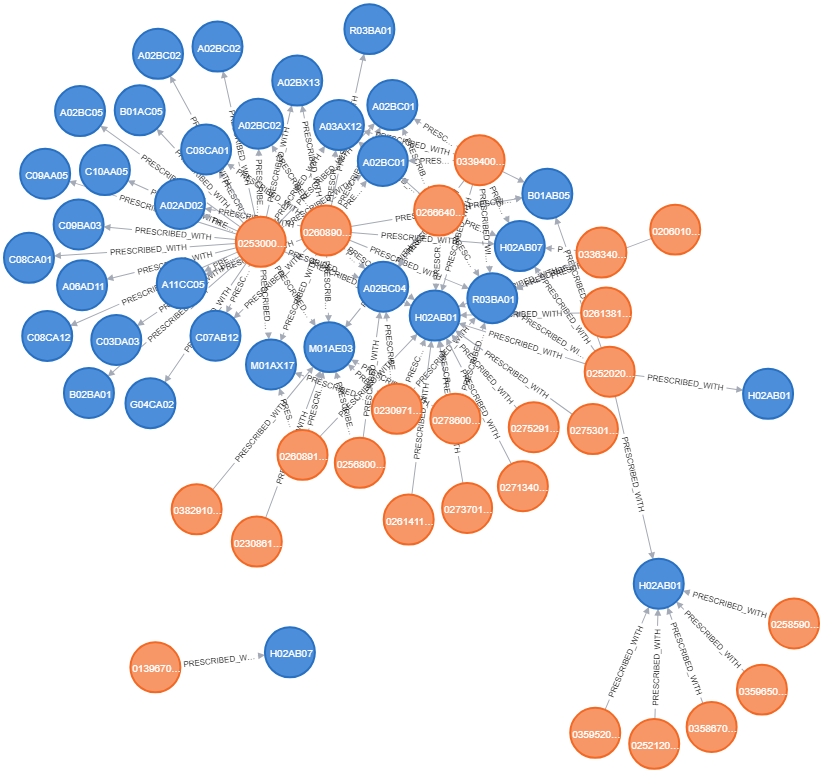
\includegraphics[scale=0.4]{./images/couples-graph.png}
\end{figure}

The component with only one couple corresponds to Plaquenil - Deltacortene, prescribed together approximately 5 000 times. Plaquenil can be used as antibiotic (antimalarial), but it is mostly given to treat arthritis, while Deltacortene is a corticosteroid for rheumatisms. 

The range of values varies from 4 145 to 38 153 in the timespan of 10 years. The 5 most popular co-prescriptions are:
\begin{enumerate}
	\item Augmentin - Oki;
	\item Rocefin - Bentelan;
	\item Augmentin - Bentelan;
	\item Normix - Cardioaspirin;
	\item Augmentin - Aulin.
\end{enumerate}

Bentelan is a corticosteroid which cannot be used without an antibiotic in presence of systemic (concerning the whole organism) infections\cite{bentelan}, since it is an immunosuppressive drug, and this would explain the frequent co-prescriptions.

All the antibiotics are among the most prescribed ones, which justifies their presence in the co-prescriptions as well.

\subsection{Projecting prescriptive habits}
Having a detailed view of doctors' most common prescriptions gives another insight on how antibiotics are related.

The three most prescribed antibiotics for each doctor are taken, along with their count, and a new relationship OFTEN\_PRESCRIBED between Doctor and Antibiotic is created. Only amounts of prescriptions greater or equal to 50 are taken into account, for consistency of results, resulting in 2 353 links.

The obtained graph displays:
\begin{enumerate}
	\item 809 doctors, the light blue nodes;
	\item 95 antibiotics, the orange nodes.
\end{enumerate}

\begin{figure}[h]
	\centering
	\includegraphics[scale=0.11]{./images/doctors-antibiotics-graph.png}
\end{figure}

Comparing the quantity of antibiotics and doctors and their relationships, it can be seen that most doctors prescribe a very restricted set of antibiotics.

To have a better understanding of the popularity of specific drugs, an auxiliary relationship PRESCRIBED\_BY\_SAME\_DOCTOR is created between Antibiotics. 

Antibiotics are interlinked with 294 new relationships:

\begin{figure}[h]
	\centering
	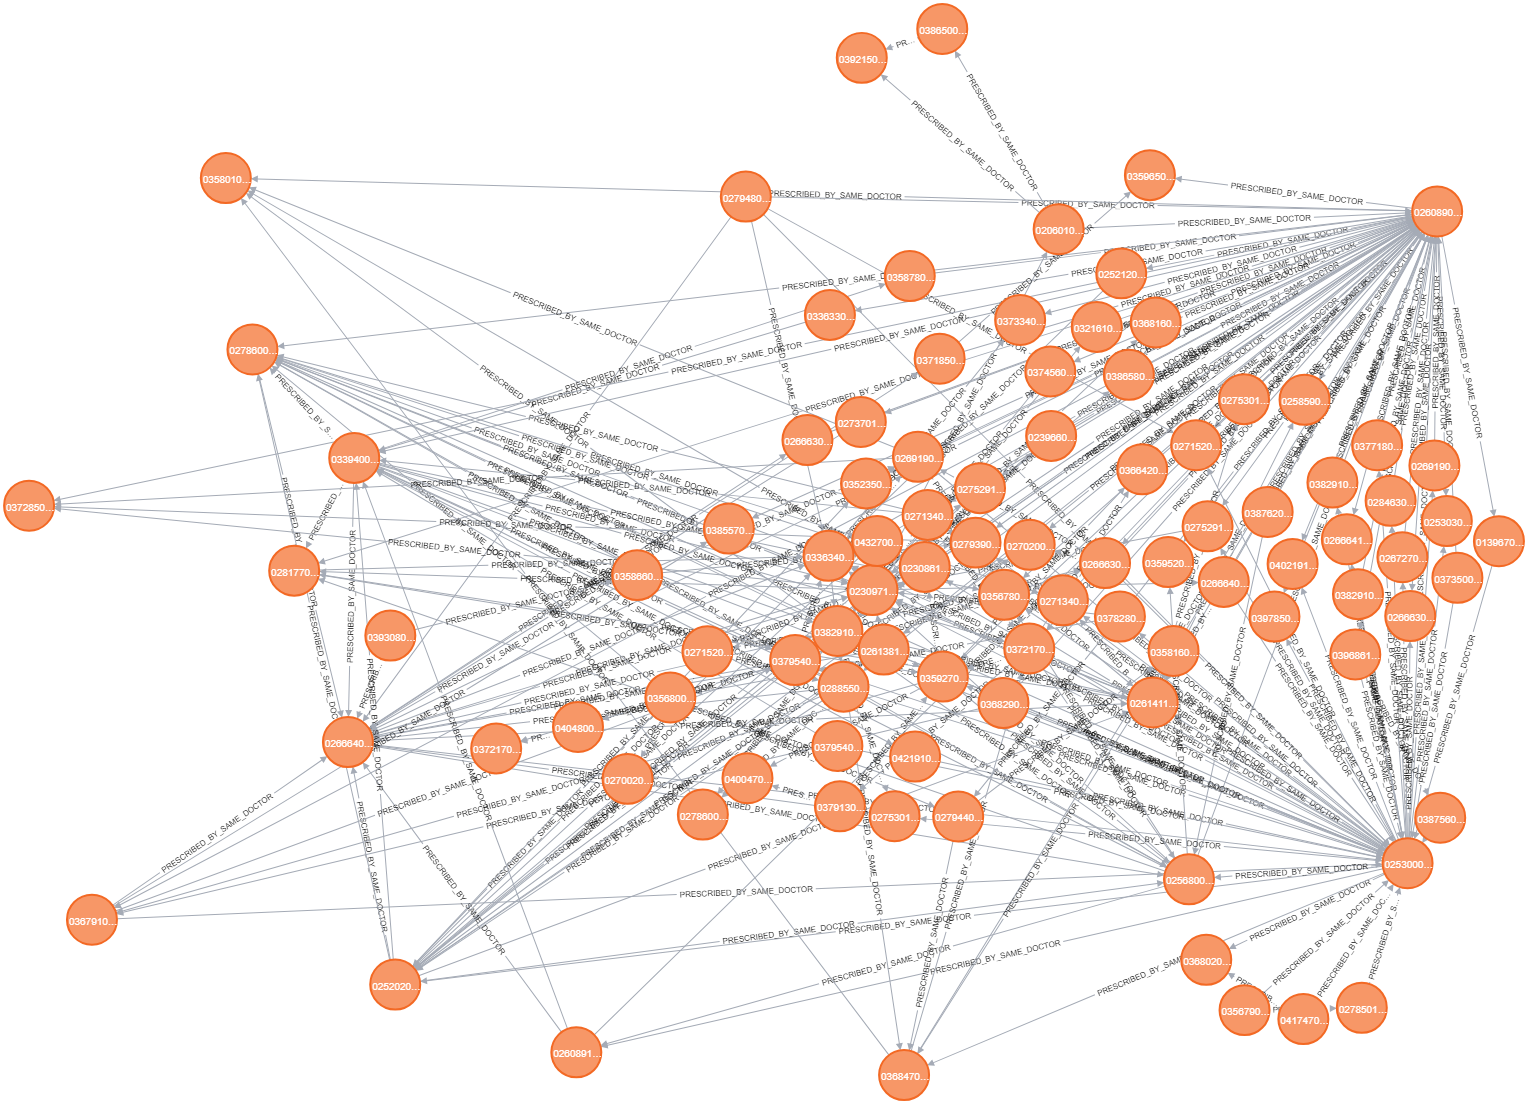
\includegraphics[scale=0.3]{./images/antibiotics-graph.png}
\end{figure}

\subsection{Centrality algorithms}

\subsubsection{Betweenness}
The Betweenness Centrality algorithm calculates the shortest (weighted) path between every pair of nodes in a connected graph, using the breadth-first search algorithm. 

Each node receives a score, based on the number of these shortest paths that pass through the node. Nodes that most frequently lie on these shortest paths will have a higher betweenness centrality score. 

Betweenness among the top 5 antibiotics:
\begin{center}
	\begin{tabular}{c|c}
		Antibiotic & Centrality \\
		\hline
		Augmentin (tablets) & 2 562 \\
		\hline
		Normix & 1 852, 74 \\
		\hline
		Velamox & 683, 78 \\
		\hline
		Ciproxin & 562, 71 \\
		\hline
		Augmentin (bottles) & 489,93 \\
	\end{tabular}
\end{center}

\subsubsection{Degree}
Degree Centrality is the simplest of all the centrality algorithms. It measures the number of incoming and outgoing relationships from a node, analysing its influence.

Degree among the top 5 antibiotics, according to co-prescriptions:
\begin{center}
	\begin{tabular}{c|c}
		Antibiotic & Degree \\
		\hline
		Augmentin (tablets) & 32 \\
		\hline
		Normix & 22 \\
		\hline
		Ciproxin & 14 \\
		\hline
		Augmentin (bottles) & 12 \\
		\hline
		Velamox & 10 \\
	\end{tabular}
\end{center}

Calculating degree among doctors is useful to determine whether the top antibiotics prescribers are also the top prescribers, using the top 5 doctors.

\begin{center}
	\begin{tabular}{c|c|c|c|c}
		Doctor & Degree (antibiotics) & Degree (medicine) & Total degree & Patients \\
		\hline
		1 & 45 625 & 51 221 & 96 846 & 4 466 \\
		\hline
		2 & 42 554 & 41 594 & 84 148 & 2 022 \\
		\hline
		3 & 35 645 & 22 383 & 58 028 & 1 816 \\
		\hline
		4 & 34 587 & 40 315 & 74 902 & 2 028 \\
		\hline
		5 & 34 380 & 28 763 & 63 143 & 1 874
	\end{tabular}
\end{center}

Seeing the obtained results, the overprescribing of some general practitioners is clear: most of them makes a number of antibiotic prescriptions equal to others having double the amount of patients.

Doctors prescribing too much and not strictly when needed is one of the main causes of antibiotic resistance in Italy.

% todo closeness?

\subsection{Community detection}
Communities are identified according to patients getting the same antibiotic or other medicine. To ease computational time, a new relationship GETS is created, with an attribute representing the number of time a patient received that determined prescription.

Since data is in the magnitude order of millions, only the top 10 most frequent antibiotics and medicines are selected. 

\subsection{Similarity detection}


\section{Considerations}







